\documentclass[11pt,a4paper]{article}
\usepackage[utf8]{inputenc}
\usepackage[T1]{fontenc}
\usepackage{amsmath,amssymb,amsfonts,amsthm,mathtools}
\usepackage{graphicx}
\usepackage[margin=1in]{geometry}
\usepackage{fancyhdr}
\usepackage{enumitem}
\usepackage{multicol}
\usepackage{xcolor}
\usepackage{tikz}
\usepackage{subcaption}
\usepackage{kotex}
\usepackage{cancel}
\usepackage[colorlinks=true]{hyperref}
\usepackage{xcolor}
\newenvironment{solution}{%
    \par\noindent\color{blue}\textbf{Answer)}\par
}{%
    \par
}

\pagestyle{fancy}
\fancyhf{}
\renewcommand{\headrulewidth}{0.4pt}
\renewcommand{\footrulewidth}{0.4pt}

\lhead{\textbf{EN5232}}
\chead{\textbf{Climate Dynamics}}
\rhead{\textbf{2026-01}}

\cfoot{-~\thepage~-}

\newcounter{question}

\newcommand{\hwquestion}[2][]{ 
  \stepcounter{question} 
  \vspace{0.6cm} 
  \noindent 
  \ifx\relax#1\relax
  \else
    {\footnotesize(#1)}\\
  \fi
  \noindent \textbf{Q\thequestion. }#2 
  \vspace{0.2cm} 
}

\newtheorem{theorem}{Theorem}[section]

\definecolor{neongreen}{RGB}{57,255,20}
\definecolor{vividmagenta}{RGB}{255,0,255}
\definecolor{brightorange}{RGB}{255,128,0}
\definecolor{vividskublue}{RGB}{0,191,255}
\definecolor{brightgold}{RGB}{255,215,0}
\definecolor{brightlime}{RGB}{191,255,0}
\definecolor{vividpurple}{RGB}{159,0,255}
\definecolor{forestgreen}{RGB}{34,139,34}
\hypersetup{
    colorlinks=true,
    linkcolor=vividskublue,
    citecolor=brightlime,
}

\begin{document}

\providecommand{\hwtitle}{Midterm}
\providecommand{\hwduedate}{2026.04.24}
\providecommand{\studentid}{20251214}
\providecommand{\studentname}{김희수}

\begin{center}
    \Large~\textbf{\hwtitle}
\end{center}

\vspace{0.4cm}

\noindent
\begin{minipage}[t]{0.5\textwidth}
Due: \hwduedate
\end{minipage}
\begin{minipage}[t]{0.5\textwidth}
    \begin{flushright}
    Student ID: \studentid\\
    Name: \studentname
    \end{flushright}
\end{minipage}

\vspace{0.4cm}
\noindent\rule{\textwidth}{0.4pt}


\hwquestion[20 pt]{How did Hadley's theory of the circulation satisfy
\begin{enumerate}[label=(\alph*)]
    \item Mass balance
\begin{solution}
Key concepts of Hadley's theory is that a single heat-driven thermally direct cell completes a full circulation from the equator to the poles. His idea takes the Earth's rotation into account.

Since the cell structure he claimed is closed, mass conservation naturally holds. 
\end{solution}
    \item Momentum balance
\begin{solution}
Absolute angular momdentum per unit mass air parcel on the rotating sphere is $$M = (u + \Omega a \cos \phi ) a \cos \phi.$$
Let the air parcel moves poleward at upper level, \textit{i.e., } $\phi \to 90^\circ$. Then in order to preserve the momentum, $\displaystyle u(\phi) = \Omega a \frac{\sin^2 \phi }{\cos \phi}$ increases which derives westerlies. 
\end{solution}
    \item In Hadley's theory, are terms such as $(u_E v_E)_Z$ necessary? Why?
\begin{solution}
No. His theory presume zonally symmetric structure of the atmospheric circulation, $(u_E v_E)_Z$ is zero. 
\end{solution}
\end{enumerate}}

\newpage
\hwquestion[20 pt]{Thermodynamic energy equation can be modified in the following steps
\[
    c_p\,\frac{d\ln\theta}{dt} = \frac{ds}{dt}
\]
where $\dfrac{d}{dt} = \dfrac{\partial}{\partial t} + \vec{V}\cdot\nabla$ with $\vec{V}$ is the 3-dimensional wind. The term $\dfrac{ds}{dt}$ is the time rate of change of entropy and is related to the rate of diabatic heating per unit mass $J$ by
\[
    J = T \left(\frac{ds}{dt}\right).
\]
\begin{enumerate}[label=(\alph*)]
    \item Starting from the above form and $T = \theta \left(\dfrac{p}{p_0}\right)^{R/c_p}$, show that
    \[
        \left(\frac{\partial}{\partial t} + u\frac{\partial}{\partial x} + v\frac{\partial}{\partial y}\right)T + T\omega\,\frac{\partial\ln\theta}{\partial p} = \frac{T}{c_p}\,\frac{ds}{dt}.
    \]

\begin{solution}
Take $\log$ on $T = \theta \left(\dfrac{p}{p_0}\right)^{R/c_p}$, then $\ln T = \ln \theta + \dfrac{R}{c_p} (\ln p - \ln p_0)$. Differentiate, then we get:
\begin{align*}
    c_p \frac{d\ln \theta }{dt} &= c_p \frac{d\ln T}{dt} - R \frac{d\ln p}{dt}\\
    &= \frac{J}{T} \quad (\because \text{Entropy form of 1st thermodynamics law}) \\
    &= \frac{ds}{dt}\\
    \Rightarrow \frac{ds}{dt} 
    &= c_p \frac{d\ln T}{dt} - R\omega \frac{\partial \ln p}{\partial p}\\
    &=  c_p \frac{d\ln T}{dt} - \frac{R \omega}{p}\\
    &= \frac{c_p}{T}\frac{dT}{dt}- \frac{R \omega}{p}\\
    &= \frac{c_p}{T} \left(\frac{\partial T}{\partial t}  + u \frac{\partial T}{\partial x}  + v \frac{\partial T}{\partial y}  + \omega \frac{\partial T}{\partial p} \right)- \frac{R \omega}{p}\\
    &= \frac{c_p}{T} \left(\frac{\partial T}{\partial t}  + u \frac{\partial T}{\partial x}  + v \frac{\partial T}{\partial y}\right)  + \frac{\omega c_p}{T}\frac{\partial T}{\partial p} - \frac{R \omega}{p}
\end{align*}
It suffices to show that $$\frac{\omega c_p}{T}\frac{\partial T}{\partial p} - \frac{R \omega}{p} = c_p \omega \frac{\partial \ln \theta }{\partial p}.$$
Again, start from the equation we take $\log$ and differentiate w.r.t $p$:
\begin{align*}
    \frac{\partial \ln T}{\partial p}&= \frac{\partial \ln \theta }{\partial p} + \frac{R}{c_p p}\\
    \Rightarrow \frac{\partial \ln \theta }{\partial p}  
    &= \frac{\partial \ln T}{\partial p}- \frac{R}{c_p p}=\frac{1}{T}\frac{\partial T}{\partial p} - \frac{R}{c_p p}\\
    \Rightarrow c_p \omega \frac{\partial \ln \theta }{\partial p} &= \frac{\omega c_p}{T}\frac{\partial T}{\partial p} - \frac{R \omega}{p}  
\end{align*}
\end{solution}


    \item Using the result in (a), $\Psi = \dfrac{\Phi}{f_0}$ and $\dfrac{\partial\Phi}{\partial p} = -\dfrac{RT}{p}$, show that
    \[
        \left(\frac{\partial}{\partial t} + u\frac{\partial}{\partial x} + v\frac{\partial}{\partial y}\right) \left(\frac{\partial\Psi}{\partial p}\right) - \frac{RT}{f_0 p}\,\frac{\partial\ln\theta}{\partial p}\,\omega = -\,\frac{RT}{f_0\, p\, c_p}\,\frac{ds}{dt}.
    \]

\begin{solution}
    From the given equations, $$\dfrac{\partial \Phi}{\partial p}= f_0 \dfrac{\partial \Psi}{\partial p}=-\dfrac{RT}{p}\Rightarrow T = -\frac{f_0 p}{R}\frac{\partial \Psi}{\partial p}.$$
    Thus, $$\left(\frac{\partial}{\partial t} + u\frac{\partial}{\partial x} + v\frac{\partial}{\partial y}\right)T=-\frac{pf_0}{R} \left(\frac{\partial}{\partial t} + u\frac{\partial}{\partial x} + v\frac{\partial}{\partial y}\right)\frac{\partial \Psi}{\partial p}.$$
    Replace the first term of (a) then we have:
         $$ -\frac{pf_0}{R} \left(\frac{\partial}{\partial t} + u\frac{\partial}{\partial x} + v\frac{\partial}{\partial y}\right)\frac{\partial \Psi}{\partial p} + T\omega\,\frac{\partial\ln\theta}{\partial p} = \frac{T}{c_p}\,\frac{ds}{dt}.$$
\end{solution}

    \item Using $\alpha = \dfrac{1}{\rho} = \dfrac{RT}{p}$, $\sigma = \alpha\,\dfrac{\partial\ln\theta}{\partial p}$, and $\vec{V} = \hat{k}\times\nabla\Psi$, derive the following equation from the result in (b):
    \[
        \frac{\partial}{\partial t} \left(\frac{\partial\Psi}{\partial p}\right) = -\,\vec{V_R}\cdot\nabla \left(\frac{\partial\Psi}{\partial p}\right) + \frac{\sigma}{f_0}\,\omega - \frac{\alpha}{f_0\, c_p}\,\frac{ds}{dt}.
    \]
\begin{solution}
    From $\vec{V} = \hat{k}\times\nabla\Psi$, compute the horizontal components:
    \begin{align*}
        \hat{k}\times\nabla\Psi 
        &= \hat{k}\times \left(\frac{\partial\Psi}{\partial x}\hat{i} + \frac{\partial\Psi}{\partial y}\hat{j}\right) \\
        &= \frac{\partial\Psi}{\partial x}(\hat{k}\times\hat{i}) + \frac{\partial\Psi}{\partial y}(\hat{k}\times\hat{j}) \\
        &= -\frac{\partial\Psi}{\partial y}\hat{i} + \frac{\partial\Psi}{\partial x}\hat{j},
    \end{align*}
    so $u = -\dfrac{\partial\Psi}{\partial y}$ and $v = \dfrac{\partial\Psi}{\partial x}$, which is the geostrophic wind $\vec{V}_R = \vec{V}_g$ since $\Psi = \Phi/f_0$. Substitute the given definitions $\alpha = \dfrac{RT}{p}$ and $\sigma = \alpha\dfrac{\partial\ln\theta}{\partial p}$ into the coefficients from (b):
    \begin{align*}
        \frac{RT}{f_0\,p}\frac{\partial\ln\theta}{\partial p} 
        &= \frac{1}{f_0}\cdot\alpha\,\frac{\partial\ln\theta}{\partial p} = \frac{\sigma}{f_0},\\
        \frac{RT}{f_0\,p\,c_p}
        &= \frac{\alpha}{f_0\,c_p}.
    \end{align*}
    Apply both substitutions to the result of (b):
    \begin{align*}
        \left(\frac{\partial}{\partial t} + u\frac{\partial}{\partial x} + v\frac{\partial}{\partial y}\right)  \left(\frac{\partial\Psi}{\partial p}\right) - \frac{\sigma}{f_0}\omega 
        &= -\frac{\alpha}{f_0\,c_p}\frac{ds}{dt}\\
        \frac{\partial}{\partial t}  \left(\frac{\partial\Psi}{\partial p}\right) + \vec{V}_R\cdot\nabla  \left(\frac{\partial\Psi}{\partial p}\right) - \frac{\sigma}{f_0}\omega 
        &= -\frac{\alpha}{f_0\,c_p}\frac{ds}{dt}\\
        \Rightarrow\;\frac{\partial}{\partial t}  \left(\frac{\partial\Psi}{\partial p}\right) 
        &= -\vec{V}_R\cdot\nabla  \left(\frac{\partial\Psi}{\partial p}\right) + \frac{\sigma}{f_0}\omega - \frac{\alpha}{f_0\,c_p}\frac{ds}{dt}.
    \end{align*}
\end{solution}

    
    \item For a state with no motion, what is the effect of increasing entropy ($\dfrac{ds}{dt} > 0$) on $T$ and $\dfrac{\partial\Psi}{\partial p}$?
    \begin{solution}
        If $u=v=\omega = 0$, (a) can be rewritten as $$\frac{\partial T}{\partial t} = \frac{T}{c_p}\frac{ds}{dt},$$ which implies $\dfrac{\partial T}{\partial t} > 0.$
        Meanwhile, from (c), 
        $$\frac{\partial}{\partial t} \left(\frac{\partial\Psi}{\partial p}\right) = - \frac{\alpha}{f_0\, c_p}\,\frac{ds}{dt}.$$ Thus, $$\frac{\partial}{\partial t} \left(\frac{\partial\Psi}{\partial p}\right) < 0.$$
    \end{solution}
\end{enumerate}}

\newpage
\hwquestion[20 pt]{Suppose the effect of the midlatitude eddies is to weaken rather than strengthen the extratropical zonal jet. More specifically, suppose that
\[
    (u_E v_E)_Z = A_0 \left(\frac{\delta}{90^\circ}\right)\exp \left\{-\left(\frac{p - 200\,\mathrm{hPa}}{50\,\mathrm{hPa}}\right)^{ 2}\right\}
\]
in midlatitudes, where $A_0$ is a positive constant, $\delta$ is in degrees, and $p$ is in $\mathrm{hPa}$.
\begin{enumerate}[label=(\alph*)]
    \item Show that $(u_E v_E)_Z$ as given above does indeed weaken the extratropical jet. You may find it useful to focus simply on the flux at $200\,\mathrm{hPa}$.
    \begin{solution}
        When $p=200\mathrm{hPa},$ the exponential term becomes 1. Thus, $(u_E v_E)_Z$ simplifies as 
        $$(u_E v_E)_Z \mid_{p=200\mathrm{hPa}} = \frac{A_0 \delta}{90^\circ}\Rightarrow\frac{\partial }{\partial y} (u_E v_E)_Z \mid_{p=200\mathrm{hPa}} = \frac{A_0}{90^\circ}\frac{\partial \delta }{\partial y} >0.$$
        This implies jet westerlies weaken at the given condtion. 
    \end{solution}

    
    \item What type of mean meridional circulation would this flux drive in midlatitudes? Direct or indirect? Why?
    \begin{solution}
        Since $\dfrac{\partial (u_E v_E)_Z}{\partial y} > 0$ at $200\mathrm{hPa}$, $\dfrac{\partial \overline{u}}{\partial t}<0. $
        To maintain thermal wind balance, a Coriolis term must compensate the eddy-induced deceleration. From the zonal-mean zonal momentum equation:
        $$\frac{\partial \overline{u}}{\partial t} = f\overline{v} - \frac{\partial (u_E v_E)_Z}{\partial y} \;\approx\; 0
            \quad\Rightarrow\quad
            f\overline{v} \approx \frac{\partial (u_E v_E)_Z}{\partial y} > 0.$$

        In the Northern Hemisphere ($f>0$), this gives $\overline{v}>0$ at $200\,\mathrm{hPa}$, i.e., poleward flow in the upper troposphere.
        
        By the zonal-mean continuity equation, $\dfrac{\partial \overline{v}}{\partial y} + \dfrac{\partial \overline{\omega}}{\partial p} = 0$, the lower branch must be equatorward, with rising on the equatorward (warm) side and sinking on the poleward (cold) side.
        
        Since warm air rises and cold air sinks, this circulation is thermally direct. 
    \end{solution}
\end{enumerate}}

\newpage
\hwquestion[45 pt]{Assume constant $f$ and $\dfrac{d\theta_0}{dz}$, and the geostrophic flow is two-dimensional ($y$--$z$), specifically $u_g = u_g(z,t)$ and $v_g = v_g(y,t)$.
\begin{enumerate}[label=(\alph*)]
    \item Starting with geostrophic and hydrostatic balance
    \[
        \vec{V_g} = \frac{1}{\rho_0 f}\,\hat{k}\times\nabla p,\qquad \frac{\partial p}{\partial z} = \frac{\rho_0 g}{\theta_0}\,\theta,
    \]
    show that the maintenance of thermal wind relationship requires
    \[
        \frac{d}{dt} \left(\frac{\partial u_g}{\partial z}\right) = -\,\frac{g}{\theta_0 f}\,\frac{d}{dt} \left(\frac{\partial\theta}{\partial y}\right).
    \]

\begin{solution}
    From geotrophic balance, we know $$\left(u_g, v_g\right) = \left(-\frac{1}{\rho_o f }\frac{\partial p}{\partial y}, \frac{1}{\rho_0 f}\frac{\partial p}{\partial x}\right).$$
        \begin{align*}
        \frac{\partial u_g}{\partial z} 
        &= -\frac{1}{\rho_0 f}\frac{\partial^2 p}{\partial z\,\partial y}\\
        &= -\frac{1}{\rho_0 f}\frac{\partial}{\partial y} \left(\frac{\partial p}{\partial z}\right) \\
        &= -\frac{1}{\rho_0 f}\frac{\partial}{\partial y} \left(\frac{\rho_0 g}{\theta}\,\theta\right) \\
        &= -\frac{g}{\theta f}\frac{\partial \theta}{\partial y}\\
        \Rightarrow\; \frac{d}{dt} \left(\frac{\partial u_g}{\partial z}\right) 
        &= -\frac{g}{\theta f}\frac{d}{dt} \left(\frac{\partial \theta}{\partial y}\right).
    \end{align*}
\end{solution}

    \item Determine the left side of the result in (a) from the momentum equation
    \[
        \frac{du_g}{dt} = f v_a.
    \]

\begin{solution}
    By taking partial differentiation w.r.t z on both side of the momentum equation, 
    $$\frac{\partial}{\partial z}\frac{du_g}{dt}
        = f\frac{\partial v_a}{\partial z} \Rightarrow\; \frac{d}{dt} \left(\frac{\partial u_g}{\partial z}\right) 
    = f\frac{\partial v_a}{\partial z}.$$
\end{solution}
    
    \item Interpret the result physically.
\begin{solution}
    Vertical wind shear of geostropic wind changes through the Coriolis torque acting on the vertical ageostrophic wind shear. That means, ageostrophic meridional circulation derives thermal wind shear. 
\end{solution}
    
\item Determine the right side of the result in (a) from the thermodynamic energy equation. Interpret the result physically.
\begin{solution}
    The adiabatic thermodynamic energy equation with basic state $\theta_0(z)$ gives
\[
\frac{D_g\theta}{Dt}+w\frac{d\theta_0}{dz}=0,
\qquad
\frac{D_g}{Dt}\equiv \frac{\partial}{\partial t}+v_g\frac{\partial}{\partial y}.
\]
Taking $\partial/\partial y$,
\[
\frac{\partial}{\partial y}\!\left(\frac{D_g\theta}{Dt}\right)
+\frac{d\theta_0}{dz}\frac{\partial w}{\partial y}=0.
\]
Expanding the first term gives
\[
\frac{D_g}{Dt}\!\left(\frac{\partial\theta}{\partial y}\right)
+\frac{\partial v_g}{\partial y}\frac{\partial\theta}{\partial y}
+\frac{d\theta_0}{dz}\frac{\partial w}{\partial y}=0.
\]
Hence
\[
-\frac{g}{\theta_0 f}\frac{D_g}{Dt}\!\left(\frac{\partial\theta}{\partial y}\right)
=
\frac{g}{\theta_0 f}\frac{\partial v_g}{\partial y}\frac{\partial\theta}{\partial y}
+\frac{g}{\theta_0 f}\frac{d\theta_0}{dz}\frac{\partial w}{\partial y}.
\]
Using
\[
\frac{\partial u_g}{\partial z}
=
-\frac{g}{\theta_0 f}\frac{\partial\theta}{\partial y},
\qquad
N^2=\frac{g}{\theta_0}\frac{d\theta_0}{dz},
\]
we obtain
\[
-\frac{g}{\theta_0 f}\frac{D_g}{Dt}\!\left(\frac{\partial\theta}{\partial y}\right)
=
-\frac{\partial v_g}{\partial y}\frac{\partial u_g}{\partial z}
+\frac{N^2}{f}\frac{\partial w}{\partial y}.
\]
    where $N^2 = \dfrac{g}{\theta_0}\dfrac{d\theta_0}{dz}$.

    The meridional gradient of vertical velocity acts on the stably stratified basic state to produce differential adiabatic warming/cooling, which changes the horizontal temperature gradient. Through thermal wind balance, this temperature-gradient tendency forces the vertical shear of $u_g$ to evolve. 
    \end{solution}
    
    \item Now use your results from (b) and (c) in (a), using a streamfunction for the ageostrophic wind: $v_a = \dfrac{\partial\Psi}{\partial z}$ and $w = -\,\dfrac{\partial\Psi}{\partial y}$. Express your result with all streamfunction terms on the left side of the equation.
\begin{solution}
Using
\[
\frac{D_g}{Dt} \left(\frac{\partial u_g}{\partial z}\right)
=
-\frac{g}{\theta_0 f}\frac{D_g}{Dt} \left(\frac{\partial \theta}{\partial y}\right),
\]
LHS from the momentum equation is: 
$$\frac{D_g}{Dt} \left(\frac{\partial u_g}{\partial z}\right) = f\frac{\partial v_a}{\partial z}.$$

From the thermodynamic equation
\[
\frac{D_g\theta}{Dt}+w\frac{d\theta_0}{dz}=0,
\]
taking $\partial/\partial y$ gives:
\[
\frac{D_g}{Dt} \left(\frac{\partial \theta}{\partial y}\right)
+\frac{\partial v_g}{\partial y}\frac{\partial \theta}{\partial y}
+\frac{d\theta_0}{dz}\frac{\partial w}{\partial y}=0.
\]
Hence
\begin{align*}
-\frac{g}{\theta_0 f}\frac{D_g}{Dt} \left(\frac{\partial \theta}{\partial y}\right)
&=
\frac{g}{\theta_0 f}\frac{\partial v_g}{\partial y}\frac{\partial \theta}{\partial y}
+\frac{g}{\theta_0 f}\frac{d\theta_0}{dz}\frac{\partial w}{\partial y}\\
&= -\frac{\partial v_g}{\partial y}\frac{\partial u_g}{\partial z}
+\frac{N^2}{f}\frac{\partial w}{\partial y}.
\end{align*}

Therefore,
\begin{align*}
    f\frac{\partial v_a}{\partial z}
&=
-\frac{\partial v_g}{\partial y}\frac{\partial u_g}{\partial z}
+\frac{N^2}{f}\frac{\partial w}{\partial y}\\
\Rightarrow
f\frac{\partial^2\Psi}{\partial z^2}
&=
-\frac{\partial v_g}{\partial y}\frac{\partial u_g}{\partial z}
-\frac{N^2}{f}\frac{\partial^2\Psi}{\partial y^2}\\
\Rightarrow N^2\frac{\partial^2\Psi}{\partial y^2}
+
f^2\frac{\partial^2\Psi}{\partial z^2}
&=
-\,f\,
\frac{\partial v_g}{\partial y}
\frac{\partial u_g}{\partial z}
\end{align*}
\end{solution}


    \item Assume that the right side of your result in (e) reaches a local minimum in the midtroposphere. Sketch the ageostrophic circulation streamlines in a $y$--$z$ cross-section along with arrows showing $v_a$ and $w$.

\begin{solution}
Let $F(y,z) := -f \dfrac{\partial v_g}{\partial y}\dfrac{\partial u_g}{\partial z}$. Then the result of (e) can be rewritten as $$N^2 \Psi_{yy}+ f^2 \Psi_{zz}= F(y,z).$$ As we assume that $F$ reaches a local minimum in the mid-troposphere, $N^2 \Psi_{yy}+ f^2 \Psi_{zz}<0\Rightarrow \Psi$ is local maximum and $v_a = \Psi_z,\, w=-\Psi_y$, resulting in counterclockwise circulation.
\begin{center}
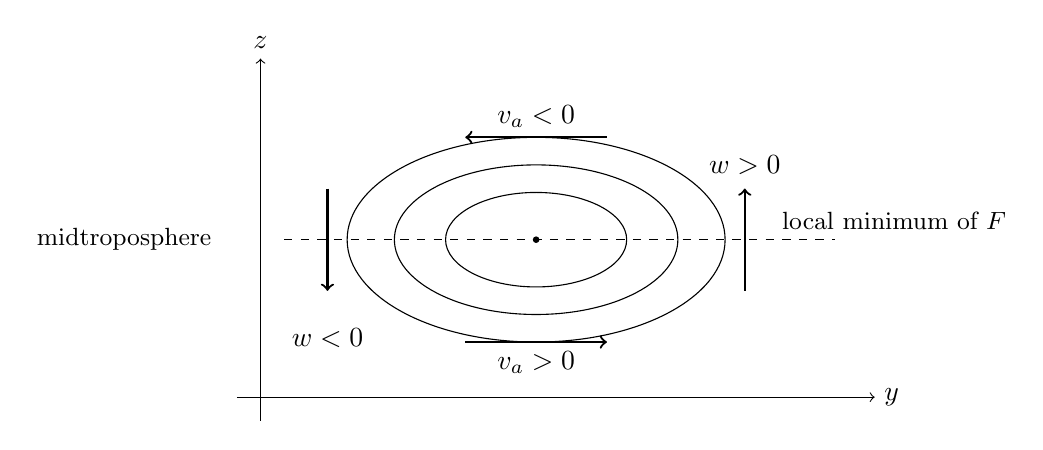
\begin{tikzpicture}[scale=1.0]
    % axes
    \draw[->] (-3.8,0.5) -- (4.3,0.5) node[right] {$y$};
    \draw[->] (-3.5,0.2) -- (-3.5,4.8) node[above] {$z$};

    % midtroposphere reference
    \draw[dashed] (-3.2,2.5) -- (3.8,2.5);
    \node[left] at (-4,2.5) {\small midtroposphere};

    % forcing minimum
    \fill (0,2.5) circle (1.2pt);
    \node[above right] at (3,2.5) {\small local minimum of $F$};

    % streamlines
    \draw (0,2.5) ellipse [x radius=2.4, y radius=1.3];
    \draw (0,2.5) ellipse [x radius=1.8, y radius=0.95];
    \draw (0,2.5) ellipse [x radius=1.15, y radius=0.60];

    % arrows showing va and w
    \draw[->, thick] (0.9,3.80) -- (-0.9,3.80);
    \node[above] at (0,3.80) {$v_a<0$};

    \draw[->, thick] (-0.9,1.20) -- (0.9,1.20);
    \node[below] at (0,1.20) {$v_a>0$};

    \draw[->, thick] (2.65,1.85) -- (2.65,3.15);
    \node[above] at (2.65,3.2) {$w>0$};

    \draw[->, thick] (-2.65,3.15) -- (-2.65,1.85);
    \node[below] at (-2.65,1.5) {$w<0$};
\end{tikzpicture}
\end{center}

\end{solution}
    
\end{enumerate}}

\newpage
\hwquestion[25 pt]{Given the following expression for the geopotential field
\[
    \Phi = \Phi_0(p) + c f_0 \left\{-\,y \left[\cos \left(\frac{\pi p}{p_0}\right) + 1\right] + \frac{1}{k}\sin k(x - ct)\right\}
\]
where $\Phi_0$ is a function of $p$ alone, $c$ is a constant wind speed, $k$ a zonal wave number, $p_0 = 1000\,\mathrm{hPa}$.
\begin{enumerate}[label=(\alph*)]
    \item Use the quasi-geostrophic vorticity equation to obtain the horizontal divergence field consistent with this geopotential field (assume $\dfrac{df}{dy} = 0$).

    \begin{solution}
        Note that QG vorticity equation is:
        $$\frac{\partial \zeta_g}{\partial t} + \vec{V_g}\cdot \nabla \zeta_g = f_0 \frac{\partial \omega}{\partial p}.$$
        \begin{align*}
            \frac{\partial \zeta_g}{\partial t} + \vec{V_g}\cdot \nabla \zeta_g 
            &= \frac{\partial }{\partial t} \left(-ck\sin \xi \right) + \vec{V_g}\cdot \nabla \zeta_g \\
            &= c^2 k^2 \cos \xi + \vec{V_g}\cdot \nabla \zeta_g \\
            &= c^2 k^2 \cos \xi + u_g \frac{\partial \zeta_g}{\partial x} + \cancelto{0}{v_g \frac{\partial \zeta_g}{\partial y} }\\
            &= c^2 k^2 \cos \xi -c^2 k^2 \left(1 + \cos \left(\frac{\pi p}{p_0}\right)\cos \xi \right)\\
            &= -c^2 k^2 \cos \left(\frac{\pi p }{p_0}\right) \cos \xi
        \end{align*}
        Since the horizontal divergence is: $\displaystyle\nabla_h \cdot \vec{V} = -\frac{1}{f_0}\left(\frac{\partial \zeta_g}{\partial t} + \vec{V_g}\cdot \nabla \zeta_g\right)$,
        \begin{align*}
            \displaystyle\nabla_h \cdot \vec{V} 
            &= -\frac{1}{f_0}\left(\frac{\partial \zeta_g}{\partial t} + \vec{V_g}\cdot \nabla \zeta_g\right)\\
            &= -\frac{1}{f_0}\left(-c^2 k^2 \cos \left(\frac{\pi p }{p_0}\right) \cos \xi\right)\\
            &= \frac{c^2 k^2}{f_0} \cos \left(\frac{\pi p }{p_0}\right) \cos k (x-ct)
        \end{align*}
    \end{solution}

    
    \item Assuming that $\omega(p_0) = 0$, obtain an expression for $\omega(x,y,p,t)$ by integrating the continuity equation with respect to pressure.
\begin{solution}
    \begin{align*}
        \frac{\partial \omega}{\partial p}
        &= \frac{1}{f_0} \left(\frac{\partial \zeta_g}{\partial t} + \vec{V_g}\cdot \nabla \zeta_g\right)\\
        &= -\frac{c^2 k^2}{f_0} \cos \left(\frac{\pi p }{p_0}\right) \cos k (x-ct)
    \end{align*}
    Integrate from $p_0$ to $p$ with initial condition $\omega(p_0)=0:$
    \begin{align*}
        \omega(x,y,p,t)
        &=  -\frac{c^2 k^2}{f_0} \cos k (x-ct) \int_{p_0}^p \cos \left(\frac{\pi p' }{p_0}\right) \, dp'\\
        &=  -\frac{c^2 k^2}{f_0} \cos k (x-ct) \left[\frac{p_0}{\pi}\sin\left(\frac{\pi p'}{p_0}\right) \right] \bigg|_{p'=p_0}^{p'=p}\\
        &=-\frac{c^2 k^2 p_0}{\pi f_0} \cos k (x-ct) \sin \frac{\pi p}{p_0}
    \end{align*}
\end{solution}
    
    \item Sketch the geopotential field at $750\,\mathrm{hPa}$ and $250\,\mathrm{hPa}$. Indicate regions of maximum divergence and convergence, along with positive and negative vorticity advection.

\begin{solution}
From the definition above, at a certain pressure level, we can find 
$$y = \frac{1}{k \left(\cos \frac{\pi p}{p_0} + 1 \right)}\sin k(x-ct) + \mathrm{const}.$$
Now, compare two pressure levels, $750\mathrm{hPa}$ and $250\mathrm{hPa}.$
\begin{align*}
    y_{750\mathrm{hPa}} &\sim \frac{1}{k \left(\cos \frac{3\pi}{4} + 1 \right)}\sin k(x-ct)\\
    &\approx \frac{1}{0.29k}\sin k(x-ct)\\
    y_{250\mathrm{hPa}} &\sim \frac{1}{k \left(\cos \frac{\pi}{4} + 1 \right)}\sin k(x-ct)\\
    &\approx \frac{1}{1.7k}\sin k(x-ct)
\end{align*}
Next, we can determine vorticity advection by measuring sign of $$-\vec{V_g}\cdot \nabla \zeta_g= c^2 k^2\left(1+\cos\frac{\pi p}{p_0}\right) \cos \xi.$$
Thus, the regions on the wave follows the order: trough $\to$ positive PV advection $\to$ ridge $\to$ negative PV advection $\to$ trough.
Lastly, the extremum of $\nabla_h\cdot \vec{V}$ left. From the results of (a) ,
$$\nabla_h\cdot \vec{V} = \frac{c^2 k^2}{f_0} \cos \left(\frac{\pi p}{p_0}\right)\cos \xi
\propto\begin{cases}
    \cos \xi & \text{at }250\mathrm{hPa}\\
    -\cos \xi & \text{at }750\mathrm{hPa}
\end{cases}.$$
Thus, the geopotential fields would be:
\begin{center}
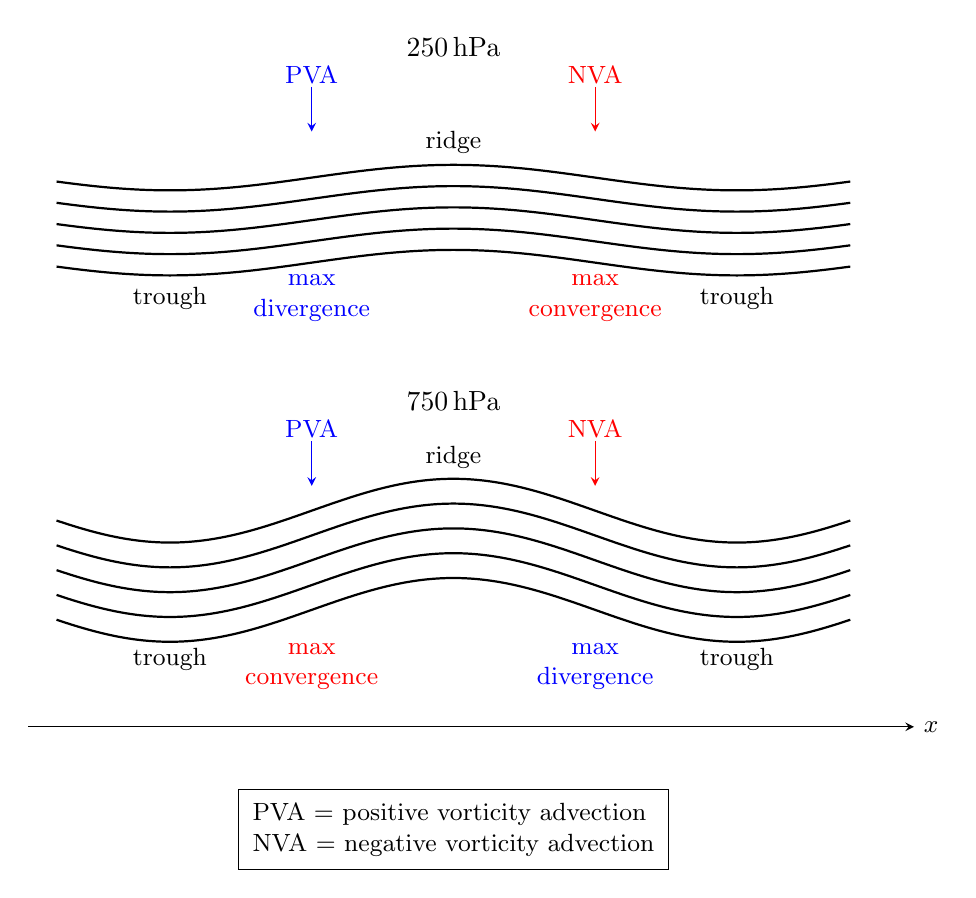
\begin{tikzpicture}[x=0.9cm,y=0.9cm,>=stealth,font=\small]

% ---------- 250 hPa ----------
\node[text=black,font=\bfseries\normalsize] at (6,10.75) {$250\,\mathrm{hPa}$};

\foreach \b in {7.70,8.00,8.30,8.60,8.90}{
    \draw[black, thick, domain=0.4:11.6, smooth, samples=120]
        plot (\x,{\b + 0.18*sin(45*(\x-4))});
}

\node[text=black] at (2.0,7.2) {trough};
\node[text=black] at (6.0,9.40) {ridge};
\node[text=black] at (10.0,7.2) {trough};

\node[text=blue] at (4.0,10.35) {PVA};
\draw[blue,->] (4.0,10.18) -- (4.0,9.55);

\node[text=red] at (8.0,10.35) {NVA};
\draw[red,->] (8.0,10.18) -- (8.0,9.55);

\node[text=blue,align=center] at (4.0,7.2) {max\\divergence};
\node[text=red,align=center] at (8.0,7.2) {max\\convergence};

% ---------- 750 hPa ----------
\node[text=black,font=\bfseries\normalsize] at (6,5.75) {$750\,\mathrm{hPa}$};

\foreach \b in {2.80,3.15,3.50,3.85,4.20}{
    \draw[black, thick, domain=0.4:11.6, smooth, samples=120]
        plot (\x,{\b + 0.45*sin(45*(\x-4))});
}

\node[text=black] at (2.0,2.1) {trough};
\node[text=black] at (6.0,4.95) {ridge};
\node[text=black] at (10.0,2.1) {trough};

\node[text=blue] at (4.0,5.35) {PVA};
\draw[blue,->] (4.0,5.18) -- (4.0,4.55);

\node[text=red] at (8.0,5.35) {NVA};
\draw[red,->] (8.0,5.18) -- (8.0,4.55);

\node[text=red,align=center] at (4.0,2) {max\\convergence};
\node[text=blue,align=center] at (8.0,2) {max\\divergence};

\draw[black,->] (0,1.15) -- (12.5,1.15) node[right,text=black] {$x$};

% ---------- Legend ----------
\node[draw=black,text=black,align=left,inner sep=5pt] at (6,-0.3) {%
PVA = positive vorticity advection\\
NVA = negative vorticity advection};

\end{tikzpicture}
\end{center}
\end{solution}
\end{enumerate}}

\newpage
\hwquestion[30 pt]{Consider the tropical Hadley circulation in northern winter, as shown in the figure below. The circulation rises at $10^\circ\mathrm{S}$, moves northward across the equator in the upper troposphere, and sinks at $20^\circ\mathrm{N}$. Assuming that the circulation outside the near-surface boundary layer is zonally symmetric (independent of $x$) and inviscid (and thus conserves absolute angular momentum about the Earth's rotation axis), and that it leaves the boundary layer at $10^\circ\mathrm{S}$ with zonal velocity $u = 0$, calculate the zonal wind in the upper troposphere at the following three locations:
\begin{solution}
From the momentum equation $$M = \Omega a^2 \cos^2 \phi + ua \cos \phi,$$
$M$ should be conserved due to the absence of friction and zonally symmetry, \textit{i.e.,} $\dfrac{DM}{Dt}=0$.
Since the initial condition wind speed $u_0$ at $10^\circ $S is zero, $$M_0 = \Omega a^2 \cos^2 10^\circ.$$
By the momentum conservation, 
\begin{align*}
M &= M_0\\
    \Omega a^2 \cos^2 \phi + ua \cos \phi 
    &= \Omega a^2 \cos^2 10^\circ\\
    \Omega a \cos \phi + u 
    &= \frac{\Omega a \cos 10^\circ}{\cos \phi}\\
    \Rightarrow u(\phi) &= \Omega a\left(\frac{ \cos 10^\circ}{\cos \phi} -\cos \phi\right)
\end{align*}
\end{solution}

\begin{enumerate}[label=(\alph*)]
    \item The equator
\begin{solution}
\begin{align*}
    u(0^\circ) &= \Omega a\left(\frac{ \cos 10^\circ}{\cos 0^\circ} -\cos 0^\circ\right)\\
    &\approx -14 \mathrm{m/s}
\end{align*}
\end{solution}

    \item $10^\circ\mathrm{N}$
\begin{solution}
\begin{align*}
    u(10^\circ) &= \Omega a\left(\frac{ \cos 10^\circ}{\cos 10^\circ} -\cos 10^\circ\right)\\
    &\approx 0 \mathrm{m/s}
\end{align*}
\end{solution}

    \item $20^\circ\mathrm{N}$
\begin{solution}
    \begin{align*}
        u(20^\circ) &= \Omega a\left(\frac{ \cos 10^\circ}{\cos 20^\circ} -\cos 20^\circ\right)\\
        &\approx 43 \mathrm{m/s}
    \end{align*}
\end{solution}
\end{enumerate}}


\newpage
\hwquestion[40 pt]{The geopotential field is expressed in the following way
\[
    \Phi = \Phi_0(p) + f_0 \left\{-\,U y + \frac{V}{k}\cos \left(\frac{\pi p}{p_0}\right)\sin k(x - ct)\right\}
\]
where $U$, $V$, and $c$ are constant speeds.
\begin{enumerate}[label=(\alph*)]
    \item Use the quasi-geostrophic vorticity equation in the pressure coordinate to obtain an estimate of $\omega$. Assume that $\dfrac{df}{dy} = \beta$ is a constant (not zero) and that $\omega$ vanishes for $p = p_0$.


\begin{solution}
Let
\[
    \xi=k(x-ct),\qquad 
    C=\cos\left(\frac{\pi p}{p_0}\right),\qquad 
    S=\sin\left(\frac{\pi p}{p_0}\right).
\]
Again from QG vorticity equation, 
$$\left(\frac{\partial }{\partial t} + \vec{V_g}\cdot \nabla \right) \zeta _g  + \beta v_g = f_0 \frac{\partial \omega}{\partial p}.$$
\begin{align*}
    f_0 \frac{\partial \omega}{\partial p}
    &= \left(\frac{\partial }{\partial t} + \vec{V_g}\cdot \nabla \right) \zeta _g  + \beta v_g \\
    &= \frac{\partial \zeta _g  }{\partial t} + \vec{V_g}\cdot \nabla \zeta _g   + \beta v_g \\
    &= -kVC\cos \xi\frac{\partial \zeta}{\partial t} + u_g\frac{\partial \zeta_g}{\partial x}   + \beta v_g \\
    &= ck^2VC\cos \xi -k^2UVC\cos\xi   + \beta VC\cos\xi\\
    &= VC \cos \xi \left[\beta - k^2 (U-c)\right]\\
    \Rightarrow \frac{\partial \omega}{\partial p} &= \frac{VC \cos \xi \left[\beta - k^2 (U-c)\right]}{f_0}
\end{align*}
Integrate from $p_0$ to $p$ where $\omega(p_0)=0$:
\begin{align*}
    \omega(p) &= \frac{V \cos \xi \left[\beta - k^2 (U-c)\right]}{f_0}\int_{p_0}^p \cos \frac{\pi p'}{p_0}\,dp'\\
    &=\frac{V p_0 \cos \xi \left[\beta - k^2 (U-c)\right]}{f_0 \pi}\sin \frac{\pi p}{p_0}
\end{align*}

\end{solution}

    \item Under the same condition, use the adiabatic thermodynamic energy equation to obtain an alternative estimate for $\omega$. Determine the value of $c$ for which this estimate of $\omega$ agrees with (a).
\begin{solution}
From the adiabatic QG thermodynamic energy equation,
\[
    \left(\frac{\partial}{\partial t}+\vec{V}_g\cdot\nabla\right)
    \frac{\partial \Phi}{\partial p}
    =
    -\sigma\omega .
\]
\begin{align*}
    -\sigma\omega
    &=
    \left(\frac{\partial}{\partial t}
    +\vec{V}_g\cdot\nabla\right)
    \frac{\partial \Phi}{\partial p} \\
    &=
    \left(\frac{\partial}{\partial t}
    +U\frac{\partial}{\partial x}\right)
    \left[
    -f_0\frac{V}{k}\frac{\pi}{p_0}S\sin\xi
    \right] \\
    &=
    f_0V\frac{\pi}{p_0}cS\cos\xi
    -
    f_0V\frac{\pi}{p_0}US\cos\xi \\
    &=
    -f_0V\frac{\pi}{p_0}(U-c)S\cos\xi.
\end{align*}
Thus,
\[
    \omega(p)
    =
    \frac{f_0V\pi}{\sigma p_0}
    (U-c)
    \sin\left(\frac{\pi p}{p_0}\right)
    \cos k(x-ct)
\]

For this to agree with the result in (a),
\begin{align*}
    \frac{Vp_0}{\pi f_0}
    \left[\beta-k^2(U-c)\right]
    &=
    \frac{f_0V\pi}{\sigma p_0}(U-c) \\
    \beta-k^2(U-c)
    &=
    \frac{f_0^2\pi^2}{\sigma p_0^2}(U-c) \\
    \beta
    &=
    \left[
    k^2+\frac{f_0^2\pi^2}{\sigma p_0^2}
    \right](U-c)\\
    \Rightarrow     c
    &=
    U
    -
    \frac{\beta}
    {k^2+\dfrac{f_0^2\pi^2}{\sigma p_0^2}}
\end{align*}
\end{solution}

    \item Under the same condition, use the omega equation in the pressure coordinate to obtain an expression for $\omega$. Verify that this result agrees with the results in (a) and (b). Sketch the phase relationship between $\Phi$ and $\omega$ at $250\,\mathrm{hPa}$ and $750\,\mathrm{hPa}$. What is the amplitude of $\omega$ if
    \[
        \beta = 2\times 10^{-11}\,\mathrm{m^{-1}s^{-1}},\ U = 25\,\mathrm{m/s},\ V = 8\,\mathrm{m/s},
    \]
    \[
        k = \frac{2\pi}{10^4\,\mathrm{km}},\ f_0 = 10^{-4}\,\mathrm{s^{-1}},\ \sigma = 2\times 10^{-6}\,\mathrm{Pa^{-2}\,m^{2}\,s^{-2}},\ p_0 = 1000\,\mathrm{hPa}?
    \]

\begin{solution}
The QG omega equation is
\[
    \left(\nabla^2+\frac{f_0^2}{\sigma}\frac{\partial^2}{\partial p^2}\right)\omega
    =
    \frac{f_0}{\sigma}\frac{\partial}{\partial p}\left[\vec{V}_g\cdot\nabla(\zeta_g+f)\right]
    -\frac{1}{\sigma}\nabla^2\left[\vec{V}_g\cdot\nabla\left(\frac{\partial\Phi}{\partial p}\right)\right].
\]
Let $\xi=k(x-ct)$, $C=\cos\left(\dfrac{\pi p}{p_0}\right)$, $S=\sin\left(\dfrac{\pi p}{p_0}\right)$, $u_g=U$, $v_g=VC\cos\xi$, and $\zeta_g=-kVC\sin\xi$, then 
\begin{align*}
    \vec{V}_g\cdot\nabla(\zeta_g+f)
    &=U\frac{\partial\zeta_g}{\partial x}+\beta v_g\\
    &=-k^2UVC\cos\xi+\beta VC\cos\xi\\
    &=VC(\beta-k^2U)\cos\xi\\
    \Rightarrow \frac{\partial}{\partial p}\left[\vec{V}_g\cdot\nabla(\zeta_g+f)\right]
    &=-\frac{\pi V}{p_0}(\beta-k^2U)S\cos\xi.
\end{align*}
    
\begin{align*}
    \vec{V}_g\cdot\nabla\left(\frac{\partial\Phi}{\partial p}\right)
    &=U\frac{\partial}{\partial x}\left[-f_0\frac{V}{k}\frac{\pi}{p_0}S\sin\xi\right]\\
    &=-Uf_0V\frac{\pi}{p_0}S\cos\xi\\
    \Rightarrow\nabla^2\left[\vec{V}_g\cdot\nabla\left(\frac{\partial\Phi}{\partial p}\right)\right]
    &=Uf_0V\frac{\pi}{p_0}k^2S\cos\xi.
\end{align*}
    
Hence,
\begin{align*}
    \left(\nabla^2+\frac{f_0^2}{\sigma}\frac{\partial^2}{\partial p^2}\right)\omega
    &=-\frac{f_0\pi V}{\sigma p_0}(\beta-k^2U)S\cos\xi-\frac{f_0\pi V}{\sigma p_0}Uk^2S\cos\xi\\
    &=-\frac{f_0\pi V\beta}{\sigma p_0}S\cos\xi.
\end{align*}
Let $\omega=WS\cos\xi$. Then we have $\displaystyle \nabla^2\omega=-k^2WS\cos\xi,\,
    \frac{\partial^2\omega}{\partial p^2}=-\left(\frac{\pi}{p_0}\right)^2WS\cos\xi.$
Thus,
\begin{align*}
    -\left[k^2+\frac{f_0^2\pi^2}{\sigma p_0^2}\right]WS\cos\xi
    &=-\frac{f_0\pi V\beta}{\sigma p_0}S\cos\xi\\
    \Rightarrow W&=\frac{\dfrac{f_0\pi V\beta}{\sigma p_0}}{k^2+\dfrac{f_0^2\pi^2}{\sigma p_0^2}}.
\end{align*}
Therefore,
\[
    \omega(p)=\frac{f_0\pi V\beta}{\sigma p_0\left[k^2+\dfrac{f_0^2\pi^2}{\sigma p_0^2}\right]}\sin\left(\frac{\pi p}{p_0}\right)\cos k(x-ct).
\]
Since $U-c=\frac{\beta}{k^2+\dfrac{f_0^2\pi^2}{\sigma p_0^2}},$ all $\omega$ we yield above are equivalent.

Next, we need to draw the phase relationship. Since $  \Phi'=f_0\frac{V}{k}C\sin\xi$ and $\omega=WS\cos\xi,$
at $250\,\mathrm{hPa}$, $\displaystyle\Phi'_{250\mathrm{hPa}}\sim\sin\xi,$ and$ \omega_{250\mathrm{hPa}}\sim\cos\xi.$ Similarly at $750\,\mathrm{hPa}$, $\Phi'_{750\mathrm{hPa}}\sim-\sin\xi,$ and $ \omega_{750\mathrm{hPa}}\sim\cos\xi.$

Now, compute the amplitude. Let $D=k^2+\dfrac{f_0^2\pi^2}{\sigma p_0^2}$. Then $D\approx 5.33\times10^{-12}\,\mathrm{/m^2}$.
Therefore,
\[
    c=U-\frac{\beta}{D}=25-\frac{2\times10^{-11}}{5.33\times10^{-12}}\approx21.25\,\mathrm{m\,/s}.
\]
The maximum amplitude is: 
\begin{align*}
    |\omega|_{\max}
    &=\frac{f_0\pi V\beta}{\sigma p_0D}\\
    &=\frac{(10^{-4})\pi(8)(2\times10^{-11})}{(2\times10^{-6})(10^5)(5.33\times10^{-12})}\\
    &\approx4.72\times10^{-2}\,\mathrm{Pa\,/s}\\
    &\approx 40.7\,\mathrm{hPa\,/day}.
\end{align*}
At $250\,\mathrm{hPa}$ and $750\,\mathrm{hPa}$, $|\omega|_{250}=|\omega|_{750}\approx3.33\times10^{-2}\,\mathrm{Pa\,/s}\approx28.8\,\mathrm{hPa\,/day}$
Thus, the phase relationship can be sketched as follows:
\begin{center}
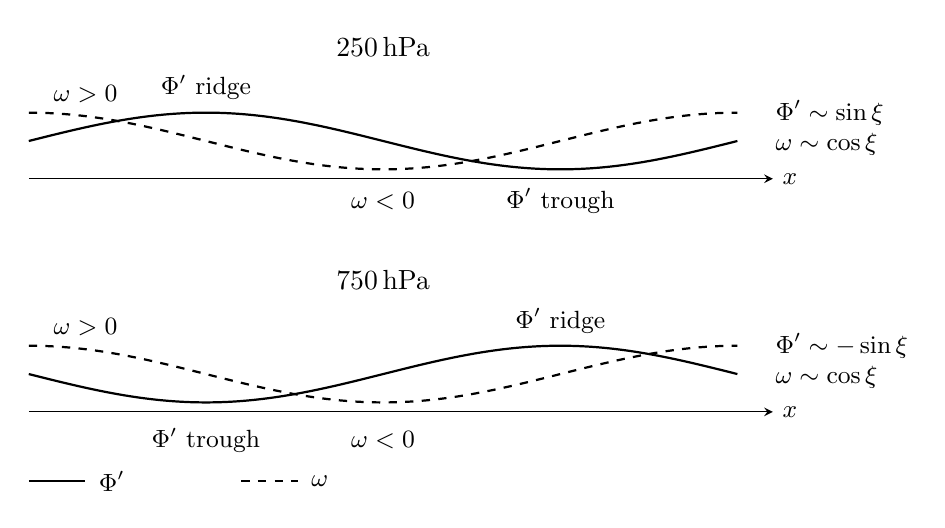
\begin{tikzpicture}[x=0.9cm,y=0.8cm,>=stealth,font=\small]

% 250 hPa
\node[font=\bfseries] at (5,4.6) {$250\,\mathrm{hPa}$};

\draw[->] (0,2.5) -- (10.5,2.5) node[right] {$x$};
\draw[domain=0:10,smooth,samples=150,thick] plot (\x,{3.1+0.45*sin(36*\x)});
\draw[domain=0:10,smooth,samples=150,dashed,thick] plot (\x,{3.1+0.45*cos(36*\x)});

\node at (2.5,3.95) {$\Phi'$ ridge};
\node at (7.5,2.15) {$\Phi'$ trough};
\node at (0.8,3.85) {$\omega>0$};
\node at (5.0,2.15) {$\omega<0$};

\node[right] at (10.4,3.55) {$\Phi'\sim\sin\xi$};
\node[right] at (10.4,3.05) {$\omega\sim\cos\xi$};

% 750 hPa
\node[font=\bfseries] at (5,0.9) {$750\,\mathrm{hPa}$};

\draw[->] (0,-1.2) -- (10.5,-1.2) node[right] {$x$};
\draw[domain=0:10,smooth,samples=150,thick] plot (\x,{-0.6-0.45*sin(36*\x)});
\draw[domain=0:10,smooth,samples=150,dashed,thick] plot (\x,{-0.6+0.45*cos(36*\x)});

\node at (2.5,-1.65) {$\Phi'$ trough};
\node at (7.5,0.25) {$\Phi'$ ridge};
\node at (0.8,0.15) {$\omega>0$};
\node at (5.0,-1.65) {$\omega<0$};

\node[right] at (10.4,-0.15) {$\Phi'\sim-\sin\xi$};
\node[right] at (10.4,-0.65) {$\omega\sim\cos\xi$};

% legend
\draw[thick] (0,-2.3) -- (0.8,-2.3);
\node[right] at (0.85,-2.3) {$\Phi'$};
\draw[dashed,thick] (3.0,-2.3) -- (3.8,-2.3);
\node[right] at (3.85,-2.3) {$\omega$};

\end{tikzpicture}
\end{center}

\end{solution}

\end{enumerate}}

\end{document}
